\documentclass[a4paper,12pt]{ltjsarticle}

% LINK
\usepackage{url}
\usepackage{hyperref}
\hypersetup{pdfborder={0 0 0.5}}

\usepackage{float}
\usepackage{setspace}
% 色の使用
\usepackage{xcolor}
% \usepackage[coloring}
\usepackage{xcolor}
\definecolor{mylinkcolor}{RGB}{3, 112, 145} %{65, 145, 3} % 色定義
\definecolor{clBlue}{RGB}{3, 112, 145} %{65, 145, 3} % 色定義
\definecolor{linkcol}{RGB}{2, 106, 77} %{65, 145, 3} % 色定義
\hypersetup{
    colorlinks=true,
    citecolor=blue,
    linkcolor=linkcol, % 
    urlcolor=mylinkcolor % 定義された色
}
% HTML(#800000)色定義
\def\colH#1{\color[HTML]{#1}}

% FONT-SIZE の定義
\def\fs#1{\fontsize{#1}{#1}\selectfont }

\usepackage[no-math,match]{luatexja-fontspec}

\usepackage{pdfpages} % 複数ページの pdf

%% 
%% POLYGLOSSIA
%% 使用の場合は%を外します
%%
% \usepackage{polyglossia}
% \setmainlanguage{churchslavonic}% 年月日をロシア語表記に
%   \setmainlanguage{japanese}
%      \setotherlanguage{russian}
%      \setotherlanguage{english}
%      \setotherlanguage{churchslavonic}
\usepackage{churchslavonic}
%%
%% CHURCHSLAVONIC:年月日
%%
\cuDefineDateFormat{long}{%
  \cuDayName{\cuDOW},
  \cuNum{\cuDAY}_гѡ~%
  \cuMonthName{\cuMONTH},~%
  лѣ́та ѿ сотворе́нїѧ мі́ра~\cuNum{\cuYEARAM}%
}

%%
%% CHURCHSLAVONIC:ドロップキャップ
%%
\usepackage{lettrine}
\makeatletter
\def\cu@lettrine{\lettrine[lines=2,findent=0pt,nindent=0pt]}
\def\cuLettrine{\cu@tokenizeletter\cu@lettrine}
\renewcommand{\LettrineFontHook}{\cuKinovarColor}
\makeatother

\usepackage{xltxtra}

\def\pkg#1{\textsf{#1}}
\def\cs#1{\texttt{\textbackslash #1}}
\def\pkg#1{\textsf{#1}}
\def\cs#1{\texttt{\textbackslash #1}}

%%
%% USER 定義
%%
\def\bs{\textbackslash}
\def\bf{\textbf}
\def\chf#1{\Ponomar{#1}}


%%
%% 欧文フォント用の設定
%%
% \setmainfont[Ligatures=TeX]{Libertinus Serif}
% \setsansfont[Ligatures=TeX]{Libertinus Sans}
\setmainfont{NotoSerif}
\setsansfont{NotoSans}
\setmonofont{RobotoMono-Light}% NotoSansMono

% \ltjdefcharrange{4}{%
% "500-"10FF, "1200-"1DFF, "2440-"245F, "27C0-"28FF, "2A00-"2AFF,
% "2C00-"2E7F, "4DC0-"4DFF, "A4D0-"A95F, "A980-"ABFF, "E000-"F8FF,
% "FB00-"FE0F, "FE20-"FE2F, "FE70-"FEFF, "10000-"1AFFF, "1B170-"1F0FF,
% "1F300-"1FFFF%, ... (and characters in U+2000–U+206F which are not in range 9)
% }% non-Japanese
%% 
%% ギリシャ文字とキリル文字
%% 
% JIS X 0208(ほとんどの和文フォント)には,これらの文字の一部が含まれている.
% • U+0370–U+03FF: Greek and Coptic
% • U+1F00–U+1FFF: Greek Extended
% • U+0400–U+04FF: Cyrillic
\ltjdefcharrange{8}{"0124,"0400-"04FF,"2626,"2720}%

%%
%% 和文フォント用の設定
%%
\newfontfamily\japanesefont[Script=Cyrillic,Ligatures=TeX]{Noto Serif CJK JP}
\newfontfamily\fNotoSerif[Ligatures=TeX]{NotoSerifJP}%FreeSerif
\newfontfamily\fNotoSans[Ligatures=TeX]{NotoSansJP}%FreeSerif
\newfontfamily\fFreeSerif[Ligatures=TeX]{FreeSerif}%
\newfontfamily\fFreeSans[Ligatures=TeX]{FreeSans}%
\newfontfamily\fRMono{RobotoMono-Light}%NotoSansMono

%%
%% キリル文字フォント用の設定
%%
\newfontfamily\cyrillicfontsf[Script=Cyrillic,Ligatures=TeX]{PomorskyUnicode}%FreeSerif
\newfontfamily\cyrillicfonttt[Ligatures=TeX]{PomorskyUnicode}
\newfontfamily\russianfont[Script=Cyrillic,Ligatures=TeX]{Linux Libertine O}
\newfontfamily\russianfonttt[Ligatures=TeX]{lmmono10-regular.otf}
\newfontfamily\russianfontsf[Ligatures=TeX]{lmsans10-regular.otf}
\newfontfamily\churchslavonicfont[Script=Cyrillic,Ligatures=TeX,HyphenChar=_]{PonomarUnicode.otf}

%%
%% fonts-churchslavonic:教会スラヴ語フォントの定義
%% /usr/share/texlive/texmf-dist/fonts/opentype/public/fonts-churchslavonic
\newfontfamily\Acathist[Script=Cyrillic,Ligatures=TeX]{Acathist-Regular.otf}
\newfontfamily\Cathisma[Script=Cyrillic,Ligatures=TeX]{CathismaUnicode.otf}
\newfontfamily\Fedorovsk[Script=Cyrillic,Ligatures=TeX]{FedorovskUnicode.otf}
\newfontfamily\Indiction[Script=Cyrillic,Ligatures=TeX]{IndictionUnicode.otf}
\newfontfamily\Menaion[Script=Cyrillic,Ligatures=TeX]{MenaionUnicode.otf}
\newfontfamily\MezenetsNo[Script=Cyrillic,Ligatures=TeX]{MezenetsUnicode.otf}
\newfontfamily\Mezenets[Script=Cyrillic,Ligatures=TeX]{MezenetsUnicode.otf}
\newfontfamily\Monomakh[Script=Cyrillic,Ligatures=TeX]{MonomakhUnicode.otf}
\newfontfamily\Oglavie[Script=Cyrillic,Ligatures=TeX]{OglavieUnicode.otf}
\newfontfamily\Pochaevsk[Script=Cyrillic,Ligatures=TeX]{PochaevskUnicode.otf}
\newfontfamily\Pomorsky[Script=Cyrillic,Ligatures=TeX]{PomorskyUnicode.otf}
\newfontfamily\Ponomar[Script=Cyrillic,Ligatures=TeX]{PonomarUnicode.otf}
\newfontfamily\Shafarik[Script=Cyrillic,Ligatures=TeX]{Shafarik-Regular.otf}
\newfontfamily\Triodion[Script=Cyrillic,Ligatures=TeX]{TriodionUnicode.otf}
\newfontfamily\Vertograd[Script=Cyrillic,Ligatures=TeX]{VertogradUnicode.otf}

\title{
    \huge {\Huge\fNotoSerif 教会スラヴ語}\\Church Slavonic Typesetting\\ in LuaTeX-ja\par\vspace{8mm}
    \Large{ [churchslavonic] } \par\vspace{120mm}
  }
  \author{\href{https://github.com/ru-museum/}{ru\_museum} (GitHub)}
\date{\today}

\begin{document}

\maketitle

 \thispagestyle{empty}

  \clearpage
  \addtocounter{page}{-2}

  \newpage

  \tableofcontents
  \thispagestyle{empty}

  \newpage

\section{概要}
\begin{itemize}
  \item これは日本語文書組版パッケージ\bf{Lua\TeX{}-ja}の\bf{ltjclasses}環境において\bf{教会スラヴ語}(\bf{Church Slavonic})の表記(含ロシア語)編集を行い、和文と露文との混在文を可能とするものです\footnote{\bf{babel}及び\bf{polyglossia}は使用していません。しかし必要に応じ使用は可能です。}。
  \item \textbf{Tex Live}付属のパッケージ\bf{churchslavonic}\footnote{Typeset documents in Church Slavonic language using Unicode.\\教会スラブ語用のフォントのインストールと、教会スラブ語及びその他の入力文字中のアンダーバー(_)のエスケイプを行います。派生的に全体に適用されエスケイプ({\colH{800000}\bs _})は不要となります。\\参照:\# texdoc churchslavonic\\\qquad\quad/usr/share/texlive/texmf-dist/doc/latex/churchslavonic/churchslavonic.pdf}を用いています。
  \item ここではキリル文字を主体とする表記の再現を目的としています\footnote{参照:\href{https://mirror.szerverem.hu/ctan/fonts/fonts-churchslavonic/docs/fonts-churchslavonic.pdf}{Church Slavonic Fonts}\\
https://mirror.szerverem.hu/ctan/fonts/fonts-churchslavonic/docs/fonts-churchslavonic.pdf}。
\end{itemize}
\vspace{-6mm}

\section{環境構築}

\subsection{動作環境}
\vspace{-2mm}
\begin{itemize}
  \item[] \textbf{GNU/Linux Debian}
  \item[] \textbf{gedit}  
  \item[] 参照:\href{https://github.com/ru-museum/lib-russian-luatexja/blob/main/lualatex-with-\qquad debian.pdf}{LuaLa\TeX{} with Debian 環境構築と作業手順}(lualatex-with-debian.pdf) 
\end{itemize}
\vspace{-8mm}
\subsection{使用パッケージ}
\vspace{-2mm}
\begin{itemize}
  \item[] \textbf{texlive}
  \item[] \textbf{texlive-lang-cyrillic}: churchslavonic  
  \item[] \textbf{texlive-fonts-extra}: fonts-churchslavonic\footnote{Fonts for typesetting in Church Slavonic language.}
\end{itemize}
\vspace{-6mm}

\subsection{教会スラヴ語用フォント}
\vspace{-2mm}
\begin{itemize}
  \item 教会スラヴ語用フォントは、以下のフォルダにインストールされています。\\
  /usr/share/texlive/texmf-dist/fonts/opentype/public/{\colH{800000}fonts-churchslavonic}
\begin{spacing}{0.58}
\begin{verbatim}
fonts-churchslavonic
 ├── Acathist-Regular.otf
 ├── CathismaUnicode.otf
 ├── FedorovskUnicode.otf
 ├── IndictionUnicode.otf
 ├── MenaionUnicode.otf
 ├── MezenetsUnicode.otf
 ├── MonomakhUnicode.otf
 ├── OglavieUnicode.otf
 ├── PochaevskUnicode.otf
 ├── PomorskyUnicode.otf
 ├── PonomarUnicode.otf
 ├── Shafarik-Regular.otf
 ├── TriodionUnicode.otf
 ├── VertogradUnicode.otf
 ├── Vilnius-Regular.otf
 └── Voskresensky-Regular.otf
\end{verbatim}
\end{spacing}
或いは以下からダウンロード出来ます。\\
\href{https://ctan.org/pkg/fonts-churchslavonic}{fonts-churchslavonic\footnote{fonts-churchslavonic – Fonts for typesetting in Church Slavonic language // CTAN\\https://ctan.org/pkg/fonts-churchslavonic}} // CTAN\\
\href{https://sci.ponomar.net/fonts.html}{Church Slavonic Fonts in Unicode}\footnote{Church Slavonic Fonts in Unicode // \href{https://sci.ponomar.net/}{Slavo­nic Compu­ting}\\https://sci.ponomar.net/fonts.html}\\
\href{http://irmologion.ru/fonts.html}{Церковно-славянские шрифты} // Ирмологий\footnote{Церковно-славянские шрифты // Ирмологий: http://irmologion.ru/fonts.html}
\end{itemize}
\vspace{-6mm}

\subsection{フォントの設定}
\begin{itemize}
  \item インストールされている{\colH{800000}fonts-churchslavonic}のフォントについては、既に設定済です。
  \item 新規インストールしたフォントを使用するには設定が必要です。\\
\textbf{設定例:}{\colH{800000}赤字}部分は自由に設定可能です。
\begin{quote}
{\fontspec{RobotoMono-Light}\bs newfontfamily\bs {\colH{800000}<Newfontname>}\{<Newfontname>.otf\}}
\end{quote}
\textbf{使用例:}
\begin{quote}
\bs{\fontspec{RobotoMono-Light}\colH{800000}<Newfontname>}
\verb+{+\Acathist{Послѣ́дованїе моле́бнагѡ пѣ́нїѧ ст҃ы̑мъ мч҃камъ к҃_гѡ вѣ́ка, въ Са́нктъ_Петербꙋ́ржстѣй дꙋхо́внѣй а҆каде́мїи нача̑льствовавшимъ, ᲂу҆чи̑вшимъ и҆ ᲂу҆чи̑вшимсѧ}\verb+}+\\[-6mm]
\end{quote}

\textbf{表示例:}
\begin{quote}
\Acathist{Послѣ́дованїе моле́бнагѡ пѣ́нїѧ ст҃ы̑мъ мч҃камъ к҃_гѡ вѣ́ка, въ Са́нктъ_Петербꙋ́ржстѣй дꙋхо́внѣй а҆каде́мїи нача̑льствовавшимъ, ᲂу҆чи̑вшимъ и҆ ᲂу҆чи̑вшимсѧ}
\end{quote}
\end{itemize}
\vspace{-6mm}

\section{編集手順}

\subsection{教会スラヴ語の表記}

\begin{enumerate}
  \item デフォルトで定義されているフォントには以下があります。\\
  但し、適正に表記されないものは除外してあります。
  \begin{table}[h]
  \begin{center}
  \begin{tabular}{l|l|l}
  \bf{定義名} & \bf{フォント名} & \bf{表記例}\\
  \hline
\bs Acathist & Acathist-Regular.otf & \Acathist{Вєсєлѧщѹ жє сѧ ѡ боѕѣ}\\
\bs Cathisma & CathismaUnicode.otf & \Cathisma{Вєсєлѧщѹ жє сѧ ѡ боѕѣ}\\
\bs Fedorovsk & FedorovskUnicode.otf & \Fedorovsk{Вєсєлѧщѹ жє сѧ ѡ боѕѣ}\\
% \bs Indiction & IndictionUnicode.otf & \Indiction{Вєсєлѧщѹ жє сѧ ѡ боѕѣ}\\
\bs Menaion & MenaionUnicode.otf & \Menaion{Вєсєлѧщѹ жє сѧ ѡ боѕѣ}\\
% \bs Mezenets & MezenetsUnicode.otf & \Mezenets{Вєсєлѧщѹ жє сѧ ѡ боѕѣ}\\
\bs Monomakh & MonomakhUnicode.otf & \Monomakh{Вєсєлѧщѹ жє сѧ ѡ боѕѣ}\\
\bs Oglavie & OglavieUnicode.otf & \Oglavie{Вєсєлѧщѹ жє сѧ ѡ боѕѣ}\\
\bs Pochaevsk & PochaevskUnicode.otf & \Pochaevsk{Вєсєлѧщѹ жє сѧ ѡ боѕѣ}\\
% \bs Pomorsky & PomorskyUnicode.otf & \Pomorsky{Вєсєлѧщѹ жє сѧ ѡ боѕѣ}\\
\bs Ponomar & PonomarUnicode.otf & \Ponomar{Вєсєлѧщѹ жє сѧ ѡ боѕѣ}\\
\bs Shafarik & Shafarik-Regular.otf & \Shafarik{Вєсєлѧщѹ жє сѧ ѡ боѕѣ}\\
\bs Triodion & TriodionUnicode.otf & \Triodion{Вєсєлѧщѹ жє сѧ ѡ боѕѣ}\\
\bs Vertograd & VertogradUnicode.otf & \Vertograd{Вєсєлѧщѹ жє сѧ}\\
  \end{tabular}
  \caption{定義されているフォントと表記例}
  \end{center}
  \end{table}
  \item 定義されているフォント名で指定します。\\
  \textbf{記述例:}\\
  {\colH{800000}\bs Monomakh}\verb+{+\Monomakh{Послѣ́дованїе моле́бнагѡ пѣ́нїѧ ...}\verb+}+\\
  \textbf{表記例:}\\
\Monomakh{Послѣ́дованїе моле́бнагѡ пѣ́нїѧ ст҃ ы̑мъ мч҃камъ к҃_гѡ вѣ́ка, въ Са́нктъ_Петербꙋ́ржстѣй дꙋхо́внѣй а҆каде́мїи нача̑льствовавшимъ, ᲂу҆ чи̑вшимъ и҆ ᲂу҆ чи̑вшимсѧ}
\end{enumerate}

\newpage

\subsection{ロシア語の表記}
\begin{itemize}
  \item 基本的にフォントの指定なしで適正表示されます。
  \item フォントの指定をする場合は、\textbf{2.4 フォントの設定}を参照して下さい。\vspace{-8mm}
\end{itemize}

\begin{quote}
\subsubsection*{フォント指定なし}
\quad Все счастливые семьи похожи друг на друга, каждая несчастливая семья несчастлива по-своему.\par
\quad Всё смешалось в доме Облонских. Жена узнала, что муж был в связи с бывшею в их доме Француженкою-гувернанткой, и объявила мужу, что не может жить с ним в одном доме. Положение это продолжалось уже третий день и мучительно чувствовалось и самими супругами, и всеми членами семьи, и домочадцами. Все члены семьи и домочадцы чувствовали, что нет смысла в их сожительстве и что на каждом постоялом дворе случайно сошедшиеся люди более связаны между собой, чем они, члены семьи и домочадцы Облонских. Жена не выходила из своих комнат, мужа третий день не было дома. Дети бегали по всему дому, как потерянные; Англичанка поссорилась с экономкой и написала записку приятельнице, прося приискать ей новое место; повар ушел еще вчера со двора, во время обеда; черная кухарка и кучер просили расчета.\par
\hspace{76mm}Анна Каренина: Л. Н. Толстой\footnote{\href{https://tolstoy.ru/online/90/18/}{Анна Каренина}: Л. Н. Толстой, Полное собрание сочинений. Том 18\\https://tolstoy.ru/online/90/18/}\par
\vspace{-6mm}

\subsubsection*{フォント指定:Linux Libertine}
\russianfont{
\quad Все счастливые семьи похожи друг на друга, каждая несчастливая семья несчастлива по-своему.\par
\quad Всё смешалось в доме Облонских. Жена узнала, что муж был в связи с бывшею в их доме Француженкою-гувернанткой, и объявила мужу, что не может жить с ним в одном доме. Положение это продолжалось уже третий день и мучительно чувствовалось и самими супругами, и всеми членами семьи, и домочадцами. Все члены семьи и домочадцы чувствовали, что нет смысла в их сожительстве и что на каждом постоялом дворе случайно сошедшиеся люди более связаны между собой, чем они, члены семьи и домочадцы Облонских. Жена не выходила из своих комнат, мужа третий день не было дома. Дети бегали по всему дому, как потерянные; Англичанка поссорилась с экономкой и написала записку приятельнице, прося приискать ей новое место; повар ушел еще вчера со двора, во время обеда; черная кухарка и кучер просили расчета.\par
\hspace{86mm}Анна Каренина: Л. Н. Толстой
}
\end{quote}
\vspace{-6mm}

\subsection{日本語の表記}
\vspace{-2mm}

\begin{itemize}
  \item 基本的にフォントの指定なしで適正表示されます。
  \item フォントの指定をする場合は、\textbf{2.4 フォントの設定}を参照して下さい。\end{itemize}
\vspace{-2mm}
\begin{quote}
\begin{spacing}{1.4}
{\fs{12pt}
\quad 日本国民は、正当に選挙された国会における代表者を通じて行動し、われらとわれらの子孫のために、諸国民との協和による成果と、わが国全土にわたつて自由のもたらす恵沢を確保し、政府の行為によつて再び戦争の惨禍が起ることのないやうにすることを決意し、ここに主権が国民に存することを宣言し、この憲法を確定する。そもそも国政は、国民の厳粛な信託によるものであつて、その権威は国民に由来し、その権力は国民の代表者がこれを行使し、その福利は国民がこれを享受する。これは人類普遍の原理であり、この憲法は、かかる原理に基くものである。われらは、これに反する一切の憲法、法令及び詔勅を排除する。\par
\quad 日本国民は、恒久の平和を念願し、人間相互の関係を支配する崇高な理想を深く自覚するのであつて、平和を愛する諸国民の公正と信義に信頼して、われらの安全と生存を保持しようと決意した。われらは、平和を維持し、専制と隷従、圧迫と偏狭を地上から永遠に除去しようと努めてゐる国際社会において、名誉ある地位を占めたいと思ふ。われらは、全世界の国民が、ひとしく恐怖と欠乏から免かれ、平和のうちに生存する権利を有することを確認する。\par
\quad われらは、いづれの国家も、自国のことのみに専念して他国を無視してはならないのであつて、政治道徳の法則は、普遍的なものであり、この法則に従ふことは、自国の主権を維持し、他国と対等関係に立たうとする各国の責務であると信ずる。\par
\quad 日本国民は、国家の名誉にかけ、全力をあげてこの崇高な理想と目的を達成することを誓ふ\footnote{「日本国憲法 前文」\\https://www.shugiin.go.jp/internet/itdb_annai.nsf/html/statics/shiryo/dl-constitution.htm}。\par}
\end{spacing}
\end{quote}

\newpage

\subsection{混在文の表記}
\vspace{-2mm}

\begin{itemize}
  \item 和文・露文共に基本的にフォントの指定なしで適正表示されます。
  \item フォントの指定をする場合は、\textbf{2.4 フォントの設定}を参照して下さい。
  \item 以下の表記例は、教会スラヴ語部分のみフォントの指定を行っています。
  \end{itemize}
\vspace{-2mm}
\hspace{12mm}\textbf{表記例:}
\vspace{-2mm}
\begin{quote}
吾輩は猫である。名前はまだ無い。\par
 どこで生れたかとんと見当がつかぬ。何でも薄暗いじめじめした所でニャーニャー泣いていた事だけは記憶している。吾輩はここで始めて人間というものを見た。しかもあとで聞くとそれは書生という人間中で一番獰悪な種族であったそうだ。この書生というのは時々我々を捕えて煮て食うという話である。しかしその当時は何という考もなかったから別段恐しいとも思わなかった。\footnote{吾輩は猫である: 夏目漱石}\par
和文の中に教会スラヴ語の記述が出来ます。
\begin{quote}
{\Monomakh Послѣ́дованїе моле́бнагѡ пѣ́нїѧ ст҃ ы̑мъ мч҃камъ к҃_гѡ вѣ́ка, въ Са́нктъ_Петербꙋ́ржстѣй дꙋхо́внѣй а҆каде́мїи нача̑льствовавшимъ, ᲂу҆ чи̑вшимъ и҆ ᲂу҆ чи̑вшимсѧ}\par
\end{quote}
ロシアの作家トルストイの小説「アンナ・カレーニナ」は、次の有名な一節で始まる。
\begin{itemize}
\item[] Все счастливые семьи похожи друг на друга, каждая несчастливая семья несчастлива по-своему.\footnote{Анна Каренина: Л. Н. Толстой}
\item[](幸福な家庭とは何れも互いに似通っているが、不幸せな家庭はそれぞれに不幸である。)
\end{itemize}
\end{quote}
\vspace{-10mm}

\section{\textbf{churchslavonic}}

\subsection{赤字表記: \fRMono\bs cuKinovar}
\vspace{-6mm}
\begin{table}[h]
\begin{center}
\begin{tabular}{l|l}
\bf{記述例} & \bf{表記}\\
\hline
{\Monomakh\verb+\cuKinovar{+ли́къ:\verb+}+ гдⷭ҇и поми́лꙋй.} & {\Monomakh\cuKinovar{ли́къ:} гдⷭ҇и поми́лꙋй.}\\
{\Monomakh\verb+\cuKinovar+ Ли́къ: гдⷭ҇и поми́лꙋй.} & {\Monomakh\cuKinovar Ли́къ: гдⷭ҇и поми́лꙋй.}\\
\end{tabular}
\caption{赤字表記}
\end{center}
\end{table}
\vspace{-10mm}

\subsection{ドロップキャップ: \fRMono\bs cuLettrine}\vspace{-2mm}

行を跨ぐ大きさ・位置は\verb+lines=+{\colH{800000}n}\verb+,findent=+{\colH{800000}0pt}\verb+,nindent=+{\colH{800000}0pt}で設定します。\\
\quad\bf{記述例:} \\
\quad\verb+\def\cu@lettrine{\lettrine[lines=+{\colH{800000}2}\verb+,findent=+{\colH{800000}0pt}\verb+,nindent=+{\colH{800000}0pt}\verb+]}+\\
\quad\verb+\Monomakh\cuLettrine{+\Monomakh{И҆́}\verb+}+\Monomakh{же дх҃а си́ла въ не́мощи соверша́етсѧ}\verb+, ...}+\\
\quad\bf{表記例:}\vspace{-9mm}
\begin{center}
\parbox{0.75\textwidth}{%
\textwidth=0.75\textwidth
\Monomakh\cuLettrine{И҆́}же дх҃а си́ла въ не́мощи соверша́етсѧ, ꙗ҆́коже пи́сано є҆́сть, и҆ вѣ́рꙋемъ: въ не́мощи же не тѣлесѐ то́чїю, но ᲂу҆́бѡ и҆ сло́ва, и҆ премꙋ́дрости на ѧ҆зы́цѣ лежа́ща. И҆ сѐ ꙗ҆́вѣ ѿ мно́гихъ ᲂу҆́бѡ}
\end{center}
\vspace{-3mm}

\subsection{年月日:}

\vspace{-6mm}
\begin{table}[h]
\begin{center}
\begin{tabular}{l|l}
\bf{記述例} & \bf{表記}\\
\hline
\verb|\cuDate{2023-8-24}| & \chf{\cuDate{2023-8-24}}\\
\verb|\cuDateJulian{2023-8-24}| & \chf{\cuDateJulian{2023-8-24}}\\
\verb|\cuDate{\cuToday}| & \chf{\cuDate{\cuToday}}\\
\end{tabular}
\caption{年月日表記}
\end{center}
\end{table}
\vspace{-14mm}

\subsection{数字}\vspace{-4mm}
\begin{table}[h]
\begin{center}
\begin{tabular}{l|l||l|l}
\bf{記述例} & \bf{表記} & \bf{記述例} & \bf{表記}\\
\hline
\verb|\cuNum{1}| & \chf{\cuNum{1}} & \verb|\cuNum{800456}| & \chf{\cuNum{800456}}\\
\verb|\cuNum{12}| & \chf{\cuNum{12}} & \verb|\cuNum{1234567}| & \chf{\cuNum{1234567}}\\
\verb|\cuNum{123}| & \chf{\cuNum{123}} & \verb|\cuNum{1500567}| & \chf{\cuNum{1500567}}\\
\verb|\cuNum{1234}| & \chf{\cuNum{1234}} & \verb|\cuNum{12345678}| & \chf{\cuNum{12345678}}\\
\verb|\cuNum{10345}| & \chf{\cuNum{10345}} & \verb|\cuNum{123456789}| & \chf{\cuNum{123456789}}\\
\verb|\cuNum{12345}| & \chf{\cuNum{12345}} & \quad & \quad\\
\end{tabular}
\caption{数字表記}
\end{center}
\end{table}
\vspace{-14mm}

\subsection{Ligatures(合字)}\vspace{-8mm}
\begin{table}[h]
\begin{center}
\begin{tabular}{l|l|c|c}
\bf{Ligature} & ユニコード & \bf{記述} & \bf{表記}\\
\hline
A-U & U+0430 U+200D U+0443 & \verb|\Ponomar{а‍у}| & \Ponomar{а‍у}\\
El-U & U+043B U+200D U+0443 & \verb|\Ponomar{л‍у}| & \Ponomar{л‍у}\\
Te-Ve & U+0442 U+200D U+0432 & \verb|\Ponomar{т‍в}| & \Ponomar{т‍в}\\
\end{tabular}
\caption{Ligature(合字)例}
\end{center}
\end{table}
\vspace{-14mm}

\newpage

\section{\textbf{fonts-churchslavonic}}

\begin{itemize}
  \item 各フォントの表記例です。
\end{itemize}
\vspace{-4mm}  

\subsection*{AcathistUnicode.otf}
\Acathist{
Бл҃же́нъ мꙋжъ,и҆́же не и҆́де на совѣ́тъ нечести́выхъ, и҆ на пꙋтѝ грѣ́шныхъ не ста̀, и҆ на сѣда́лищи гꙋби́телей не сѣ́де: но въ зако́нѣ гдⷭ н҇ и во́лѧ є҆ гѡ̀, и҆ въ зако́нѣ є҆ гѡ̀ поꙋчи́тсѧ де́нь и҆ но́щь. 
}

\subsection*{FedorovskUnicode.otf}
\Fedorovsk{
Бл҃же́нъ мꙋжъ,и҆́же не и҆́де на совѣ́тъ нечести́выхъ, и҆ на пꙋтѝ грѣ́шныхъ не ста̀, и҆ на сѣда́лищи гꙋби́телей не сѣ́де: но въ зако́нѣ гдⷭ н҇ и во́лѧ є҆ гѡ̀, и҆ въ зако́нѣ є҆ гѡ̀ поꙋчи́тсѧ де́нь и҆ но́щь. 
}

\subsection*{MenaionUnicode.otf}
\Menaion{
Бл҃же́нъ мꙋжъ,и҆́же не и҆́де на совѣ́тъ нечести́выхъ, и҆ на пꙋтѝ грѣ́шныхъ не ста̀, и҆ на сѣда́лищи гꙋби́телей не сѣ́де: но въ зако́нѣ гдⷭ н҇ и во́лѧ є҆ гѡ̀, и҆ въ зако́нѣ є҆ гѡ̀ поꙋчи́тсѧ де́нь и҆ но́щь. 
}

\subsection*{PochaevskUnicode.otf}
\Pochaevsk{
Бл҃же́нъ мꙋжъ,и҆́же не и҆́де на совѣ́тъ нечести́выхъ, и҆ на пꙋтѝ грѣ́шныхъ не ста̀, и҆ на сѣда́лищи гꙋби́телей не сѣ́де: но въ зако́нѣ гдⷭ н҇ и во́лѧ є҆ гѡ̀, и҆ въ зако́нѣ є҆ гѡ̀ поꙋчи́тсѧ де́нь и҆ но́щь. 
}

\subsection*{PonomarUnicode.otf}
\Ponomar{
Бл҃же́нъ мꙋжъ,и҆́же не и҆́де на совѣ́тъ нечести́выхъ, и҆ на пꙋтѝ грѣ́шныхъ не ста̀, и҆ на сѣда́лищи гꙋби́телей не сѣ́де: но въ зако́нѣ гдⷭ н҇ и во́лѧ є҆ гѡ̀, и҆ въ зако́нѣ є҆ гѡ̀ поꙋчи́тсѧ де́нь и҆ но́щь. 
}

\subsection*{ShafarikUnicode.otf}
\vspace{-2mm}
\Shafarik{
Бл҃же́нъ мꙋжъ,и҆́же не и҆́де на совѣ́тъ нечести́выхъ, и҆ на пꙋтѝ грѣ́шныхъ не ста̀, и҆ на сѣда́лищи гꙋби́телей не сѣ́де: но въ зако́нѣ гдⷭ н҇ и во́лѧ є҆ гѡ̀, и҆ въ зако́нѣ є҆ гѡ̀ поꙋчи́тсѧ де́нь и҆ но́щь. 
}
\vspace{-4mm}

\subsection*{TriodionUnicode.otf}
\vspace{-4mm}
\Triodion{
Бл҃же́нъ мꙋжъ,и҆́же не и҆́де на совѣ́тъ нечести́выхъ, и҆ на пꙋтѝ грѣ́шныхъ не ста̀, и҆ на сѣда́лищи гꙋби́телей не сѣ́де: но въ зако́нѣ гдⷭ н҇ и во́лѧ є҆ гѡ̀, и҆ въ зако́нѣ є҆ гѡ̀ поꙋчи́тсѧ де́нь и҆ но́щь. 
}
\vspace{-6mm}


\section{\textbf{TIPS}}
\vspace{-2mm}

\subsection{文字のエラー表示}
\vspace{-4mm}

\begin{itemize}
  \item 文字或いは約物\footnote{\Monomakh{☦}等。}等が \raisebox{-0.6ex}{
\includegraphics[width=4mm]{./images/error.png}} とエラー表示される場合、当該文字記号が使用フォントに収録されているかをフォントビューワーで調べ、あればそのユニコードをプリアンブルに追加します。\\
\vspace{-8mm}  
\begin{figure}[H]
\centering
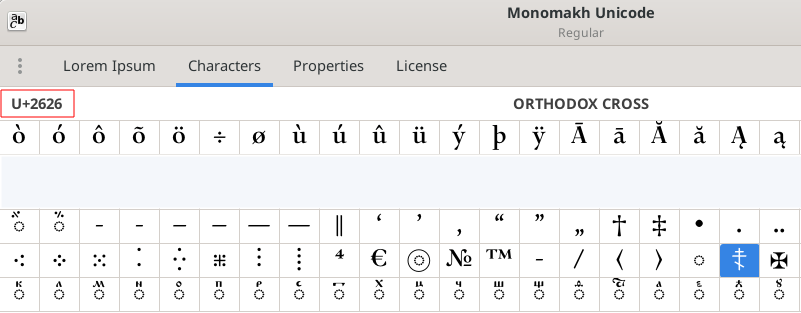
\includegraphics[width=14cm]{./images/sample-symbol.png}  
\caption{フォントビューワーで調べる} 
\end{figure}
\vspace{-10mm}  

\begin{table}[h]
\begin{center}
\begin{tabular}{c|c|c}
\bf{文字・記号} & \bf{ユニコード} & \bf{記述}\\
\hline
\Shafarik{☦} & U+2626 & {\colH{800000}"2626}\\
\end{tabular}
\caption{記述するコード}
\end{center}
\end{table}
\vspace{-6mm}  

  \verb+\ltjdefcharrange{8}{"0400-"04FF+\footnote{ユニコードにおけるキリル文字の領域。}\verb+,+{\fRMono\colH{800000}"2626}\verb+,"2720}+
  \item 或いは他のフォントを指定すると表示されることがあります。
\end{itemize}

\end{document}





